%%This is a very basic article template.
%%There is just one section and two subsections.
\documentclass[12pt,paper=a4,nenglish]{scrreprt}

\setlength{\parindent}{0pt}

\usepackage{babel}
\usepackage[T1]{fontenc}
\usepackage[utf8]{inputenc}

\usepackage{geometry}
\geometry{includefoot, a4paper, left=30mm, right=25mm, top=25mm, bottom=15mm}
\usepackage[small,sf,bf,hang]{caption}

\usepackage{setspace} % for onehalfspacing
\usepackage{titlesec}
\usepackage{graphicx}
\usepackage{float}
\usepackage{cite}

\titlespacing*{\chapter}{0pt}{-30pt}{20pt}
\titleformat{\chapter}
  {\normalfont\sffamily\Large\bfseries}
  {\thechapter}{14pt}{}
\titleformat{\section}
  {\normalfont\sffamily\large\bfseries}
  {\thesection}{12pt}{}

\usepackage{color}
\usepackage[table]{xcolor}
  
\usepackage{lmodern}
\definecolor{darkgray}{rgb}{0.8,0.8,0.8}
\definecolor{lightgray}{rgb}{0.95,0.95,0.95}
\definecolor{lightergray}{rgb}{0.97,0.97,0.97}

%\makeatletter
%\renewcommand\@makefntext[1]{\leftskip=2em\hskip-2em\@makefnmark#1}
%\makeatother
\usepackage[hang,flushmargin]{footmisc}
\usepackage{listings}


\begin{document}
\thispagestyle{empty}
\begin{center}
\textbf{\sffamily	Universität Leipzig\\
			Institut für Informatik \\
			Digital Humanities\\}
\end{center}

\begin{center}
\vspace{4cm}
{\textbf{\sffamily Final Write Up }}
\end{center}

\begin{center}
	\vspace{0.5cm}
	{\sffamily Freie wissenschaftliche Arbeit \\
			   im Rahmen des Fachs "`Digital Philology"' \\ 
	           an der Fakultät für Mathematik und Informatik der Universität
	           Leipzig  }
\end{center}

%Thema: 

\begin{center}
	\vspace{1cm}
	\textbf{\sffamily Conclusion on the project work of digital philology }\\
	\vspace{2.5cm}
\end{center}
\vfill

\begin{center}
	{\large
	\begin{tabular}{p{7cm} l}
	
	\small Betreuender Hochschullehrer:		&\small Prof. Dr. Crane\\
	\small Betreuender Assistent: 	 		&\small Matt Munson\\
	\small Verfasser: 						&\small Alexander Richter, Dan Häberlein,  \\
											& \small Nathanael Phillip, Peggy Lucke\\
											& \small MatNr. 2517643\\
											& \small M.Sc. 2. Semester\\
											& \\
	\small Eingereicht am: 					& \small \today
	
	\end{tabular}}
\end{center}
\renewcommand*\contentsname{Table of contents}
\tableofcontents
\onehalfspacing

\setcounter{page}{1} 
\chapter{Introduction}
In this essay the project work 'Open Legislature' will be discussed, which was
created during the subject 'Digital Philology' in the summer term 2014.
The goal of this essay is to present our results in an understandable fashion,
reflecting the way we produced our results. 
In course of this work all our created (software) artifacts and analysed results
regarding politicians of the german Bundestag should be presented.
We begin with a short introduction of our posed questions and the corpus which
was used trying to answer them. Afterwards we talk about simple
misunderstandings of the problem space. 
In the next chapter we will talk
about our methodology, software artifacts and achieved results.
Finally, we conclude this work with a critical reflection of your own research
process, namely what we did right and wrong during the last term.
\section{Questions}
At first we wanted to know: Can it be detected, if some politicians
use a ghost writer? Or is it possible, that even politicians from different
parties have the same ghost writer? \\ 
Those questions are based on the fact that in your digital world it
seems kind of easy to copy the work of others or even assign someone else to do
your work. For reference, this article \cite{plagiat_1} of a german online newspaper 
summarises current plagiarism cases of many german politicians. 
Even Wladimir Putin, the current president of the Russian Federation, has been
suspected cheating in his dissertation \cite{plagiat_2}. This has been in
2006. \\
Another interesting story can be told of an software developer from the USA,
who 'outsourced' all of his personal work to a company in china
\cite{plagiat_3}. In return, he transfered the half of his salary to the chinese
cooperation. He was free to do whatever he wanted in the office, spending the
most of his day to watch cat videos or surfing on social networks. 
On top of that, before anyone noticed, he has been honored as 'one of the best
employes of his department'. \\
Those examples should illustrate that copying is all around us. 
It is kind of unfair, because there are many people who have to work hard and on
their own to reach their goals. We should have some tools, to be able to detect plagisms.\\
A whole other dimension of the original issue is the political side. In your
modern parliamentary democracies, we need to trust the elected
politicians. Who has time to really follow their debates? If we can not or
want not to change the political system, at least the majority should have the
right of information and transparency. And computer science can help us to achieve this.
\\
As expected, the current presented questions were not easy to
answer. We also did not find any data about ghost writers for german
politicians (which should be self evident), only the speeches they gave in the
parliaments.
Therefore, we had to abandon this really interesting questioning. As
we discuss later in the conclusion chapter, we contradicted the scientific
approach to answer questions: We tried to find questions considering our data. 
For example we compared speeches of different politicans to find similarities
in there speeches, which can be interesting, but without a concreate set of
questions it may not be expedient.  
So we redefined our main question to be: 'What are typical used words for a
specific politician? Which politicians use similar words?'. 
%Also interesting
%could have been 'What are the important words of a time period?'.
The corpus, luckily, was capable to answer many meaningful questions. But
theoretically speaking, we had a basic problem in our methology: Finding questions for a
dataset. 

\section{Corpus}
During the first couple of weeks in our digital humanities course, we were
asked to search for data which can be used for linguistic analysis.
We should have collected more data regarding the original questioning. But we
did not find any obvious hints for ghostwriting in the german
parliament (Bundestag). 
As already mentioned, we only found the official records of the german
parliament.
For every session of the Bundestag, all stenographic reports are freely
available \cite{link_plenarprotokolle}. All 'protocols' of the Bundestag since the founding of the German Federal Republic
(1949) are extractable in the pdf format. In total, there are about 4000 PDF
documents for all sessions and election periods. 
They make up a dataset of nearly 10 GB. 
For our analysis, we used this dataset exclusively. 
\section{Understanding the problem}
\label{sec:understanding_the_problem}
As computer scientists we were not used to linguistic questions.
During the course we learned a bit too late what should be asked and what is
not answerable easily. That is most likely one of the reasons we came up with
typical data and statistical results (like for decision support systems in an enterprise). 
Another point is that computer scientists produce software and tools sometimes
way too early. They should concentrate on their goals, achieving results (so in
this case the answers of our questions) in the most simple fashion. I think we
did use too complicated approaches, which did not show any results so quickly,
frustating the whole team. For example, we had a document pipeline to extract
all Bundestag protocols from the internet. Instead of reducing the dataset by
selecting only protocols of one period we invested time to make the process
parallel. Of course this was  helpful, but did not produce any answers. If we
would have already finished for a small subset (maybe the current
election period), we could have implemented this feature. But
before that it was just a waste of time.

\chapter{Our Achievements}
In this chapter we will talk about our results
and describe how anyone could reproduce them. The main goal is to express what
we have done and how. At first we will show the timeline of the
last term and what was done when giving also an overview over the produced
artifacts.
Then we go over every artifact in detail, reflecting
our work critically. 
\section{Artifact Overview}
\label{sec:artifact_overview}
As results in any form, we created the following during the last term:
\begin{itemize}
  \item A Java application called 'document pipeline' to extract and process
  all Bundestag protocols of the past and the future. 
  This application has been designed to extract the text from the protocols
  using an optical character regocnition library. Afterwards we were using it
  to create structured data from each protocol.
  \item Using the data created by our document pipeline, we were able to
  build an easy website providing adhoc analysis of the data. We call this
  module 'Data visualization'. We also provide our later results of the SLDA
  Classification on this
  website.%??????????????????????????????????
  \item In our intention to group speeches by topics we used the SLDA
  classification algorithm. We had really problems to use it on such an
  overwhelming amount of data. 
  \item We created a meta database using a graph database (Neo4J). This
  database concludes information about the composition of the Bundestag of
  every election period, the detailed numbers of how many mandats each parties
  got, which parties form the gouvernment coalition and so on. 
\end{itemize}
In the last term during our digital humanities course we had to master a great
amount of workload. For every group member, there should have been about 8 hours
per week spending on the group project. We did our best, but we think the whole
project was a bit too heavy for a 10 ECTS course (although this time is ensured
by 10 ECTS course). 
Furthermore, we should have had a clear finishing
date (not vaguely by the end of the term). In the following figure
\ref{pic:timeline}, we want to show what we have done and how much time we spent
for it. Notice that we misestimated quite often how long we needed for a
feature, which took many time from our project. For each artifact we will talk about the misestimation in
detail in their associated chapters.
\begin{figure}[H] 
	\centering
	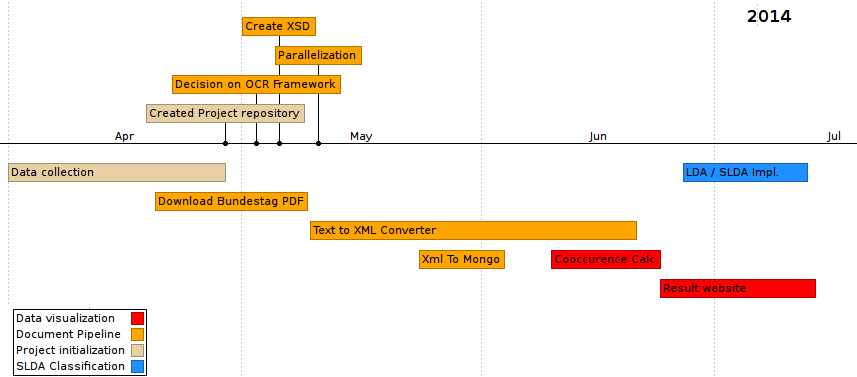
\includegraphics[scale=0.7]{res/timeline_term.png}
	\caption{Timeline of the Open Legislature project during summer term 2014}%
	\label{pic:timeline}%
\end{figure}%
Roughly speaking we spent more than the half of the term on implementing
the document pipeline, followed in terms of effort by our result visualization
module and the LDA / SDLA calculation. Alone judging by the time taken, it was
most complicated to transfer the unstructured PDF protocols into a more machine
readable format. We will talk about this process in the next part of this essay. 

\section{Document Pipeline} 
From the perspective of our project github repository, we are now going to
explain the content of the openLegislature folder. This is shown in figure
\ref{pic:doc_pipeline_github}: 
\begin{figure}[H] 
	\centering
	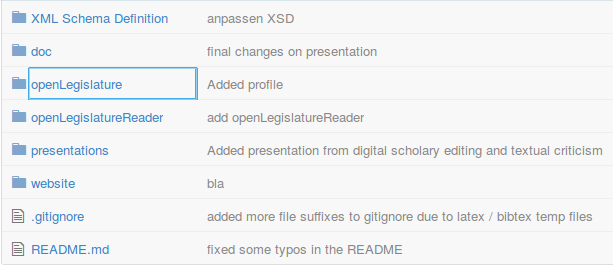
\includegraphics[scale=0.7]{res/document_pipeline.png}
	\caption{Document pipeline folder in the project github repository.}%
	\label{pic:doc_pipeline_github}%
\end{figure}%
As already in chapter \ref{sec:understanding_the_problem} and
\ref{sec:artifact_overview} introduced, we created an Java application which
converts the unstructured Bundestag protocols in pdf format into structured
data. This data will be stored into a database called 'Mongo DB' (a
schemaless document oriented database with a powerfull query language with
similar functionalities to SQL). \\
This Java project is organized with Maven. 
Maven is a simple tool to create (compile, resolve third party libraries,
execute) Java applications. Concluding these points, we can state the
prerequisites of our document pipeline if you want to build and run it:
\begin{itemize}
  \item Java JDK 7 or later
  \item Maven 3
  \item MongoDB (running instance on default port 27017) 
\end{itemize}
Then just clone the repository and issue the following command in the
'openLegislature' folder (the folder shown in graphic
\ref{pic:doc_pipeline_github}) to build and run all of our Java applications
(the document pipeline AND the SLDA transformation):
\begin{description}
	\lstinputlisting[tabsize=2, captionpos=b, frame=single, numbers=none,
	language=bash, caption=Maven command to build and execute the
	document pipeline]{res/maven_build_all.sh} \label{listing:maven_build_comman.}%
\end{description}
This command can take some time to execute, because it will download, process
and insert all Bundestag protocols available. There are some command line
parameters which can be added to the Maven call using '-Dopenlegislature.XXX',
enabling fine grained settings, e.g. the reduction of loaded protocols (for example
to select on a different election period range). For more information please consult the appendix
\ref{appendix:document_pipeline_parameters}. \\
 
The document pipeline module works for over 90\% of the protocols. For the
others, our problem module, the text to xml parser, does not generate valid xml.
As illustrated in figure \ref{pic:timeline}, this part of the document pipeline
took the most time. We misestimated the effort of the text to xml parser. For
example, during the different election periods, the structure of the
protocols changed. This knowledge had to be gained manually reading the
protocols, transfering it into the source code of the text to xml parser. An
idea for comparable future work is to invest much more time into the analysis of
the differnt types of text (pdf) files and categorizing them. But still it would
not be easily possible to produce 100 \%, because exceptions do occur.  
If there is not much time and when focusing on
results, it is usally also a good idea to reduce the dataset.\\ 
The text to xml parser should also be created with an API (like
lxml in python or the xerces DOM implementation in Java) to ensure valid xml documents. It was created with simple strings, which caused us large maintenance overhead. \\
Another issue from the organizing perspective was the design of our process. We
first thought, that xml will solve all our problems and structures the data
enough. We could have used XPath or XQuery as powerful query languages. As we
moved on to the data visualization part, it turned out that a database
handeling the content of our protocols could be a better choice regarding
more convenient queries. So we transfered our data from files to Mongo DB. This
was just a step for convenience. We could have worked with XPath as well. This took not so long,
but we spent again some time there.\\
To finish this part, our results of the shown software should be emphasized: We
have a program, that can download all of the Bundestag protocols, convert those
pdfs to text, convert again the text to xml and finally insert this xml into Mongo DB. 
We have now structured data which can be analysed much easier. 
\section{Data visualization}
This module was called data visualization, although we also analysed parts of
our created dataset (we calculate cooccurences of words in different speeches,
the log likelihood for them, etc). For our github repository, the artifacts for this
module are located as shown in figure \ref{pic:doc_visualization}. 
\begin{figure}[H] 
	\centering
	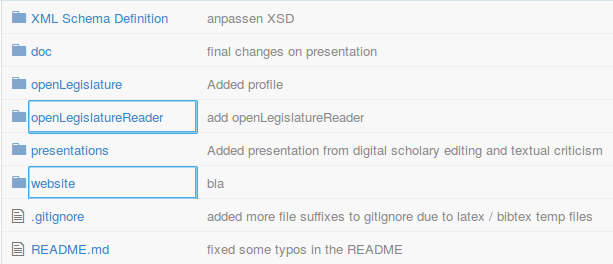
\includegraphics[scale=0.7]{res/visualization_folder.png}
	\caption{Analasys and visualization modul folder in the project github
	repository.}%
	\label{pic:doc_visualization}%
\end{figure}%
In the 'openLegislatureReader' folder we created an Java application which read
our Mongo DB database, calculating for all speeches cooccurence matrices. For simplicity,
we wrote this data back into Mongo DB. Because this calculation also took very
long, we provide the data in the json format for importing, sparing anyone the
long calculation time. There are: 	
\begin{itemize}
  \item ollspeeches.json
  \item partystats.json
  \item plenarprotokolle.json
  \item speakerstats.json
\end{itemize}
containing our results for the visualization website. We would have
provided those files using github, but they are too large to upload. Instead, we
put them into a cloud service repository called 'Copy'. In this moment 
those files are not open to the public because
of their size. Of course they are
retrievable from us. \\ 
When the data has been imported successfully, you finally need to install our
result webpage. The orignal idea was to publish the page on the internet, but
unfortunately we didn't have an own webserver and domain with the capabilities
to hold our data. Therefore, it must be installed on your machine.
In total, for running the data visualization module you need:
\begin{itemize}
  \item Webserver (e.g. apache2)
  \item PHP (The used language for the server side)
  \item The Mongo DB driver for PHP
\end{itemize}
For example on Linux / Unix, you can retrieve those dependencies using your
system's package manager. Afterwards, copy the 'website' folder from figure
\ref{pic:doc_visualization} of our github repository into the root folder of
your webserver (e.g. /var/www for apache2). When all is well
installed, Mongo DB is running and the data is properly imported you can access our result webpage using the URL given by listing
\ref{listing:url_of_website}.
\begin{description}
	\centering
	\lstinputlisting[tabsize=2, captionpos=b, frame=single, numbers=none,
	language=bash, caption=URL for the browser of the data
	visualization module]{res/url_to_website.txt}
	\label{listing:url_of_website}%
\end{description}
You should see a webpage comparable to this, illustrated in figure \ref{pic:website}: 
\begin{figure}[H] 
	\centering
	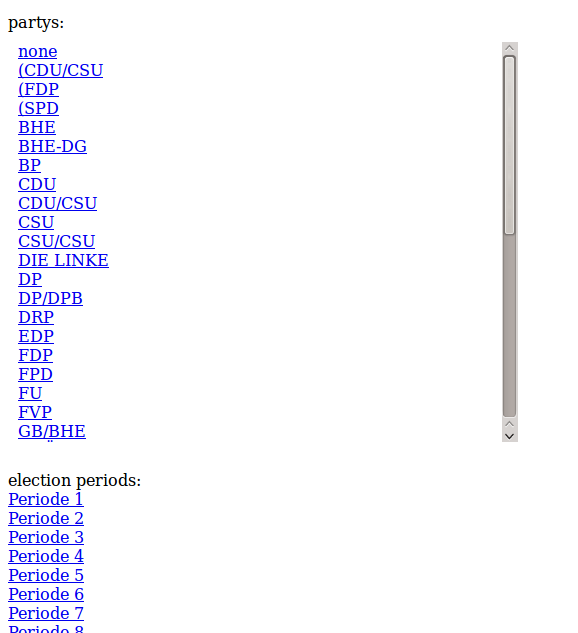
\includegraphics[scale=0.4]{res/website_view.png}
	\caption{Data visualization website}%
	\label{pic:website}%
\end{figure}%
We assume that the user interface is really minimal, but you should get a good
first idea what the data looks like. Using the webpage, we can infer many
metrics about the data for speakers, parties and election periods. 
One interesting diagram type shows the top words of a politician. In
figure \ref{pic:wagenknecht_topwords}, we show an example for Dr. Sarah
Wagenknecht (member of the party Die Linke):
\begin{figure}[H] 
	\centering
	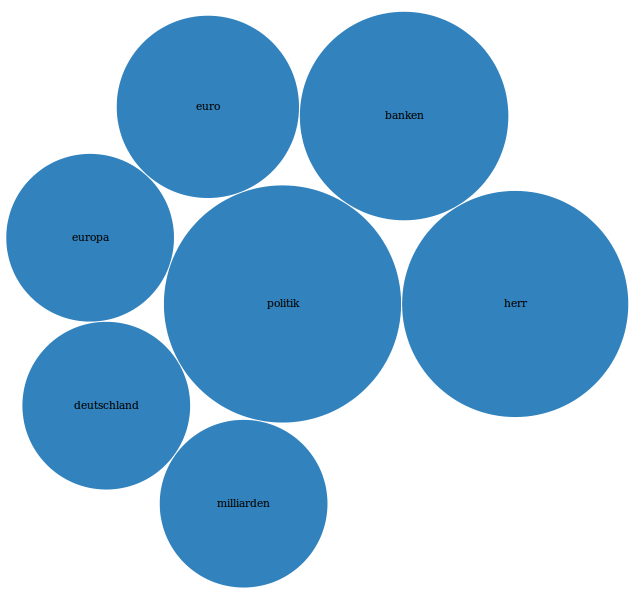
\includegraphics[scale=0.6]{res/wagenknecht_topwords.png}
	\caption{Top used words by Dr. Sarah Wagenknecht (without stopwords)}%
	\label{pic:wagenknecht_topwords}%
\end{figure}%
We deleted any stopwords using a stopword list to elimate typical german words
without a deeper meening. As you can see, Dr. Sarah Wagenknecht talks in her
speeches much about euro politics. Such insights can be performed for every
speeker of the german Bundestag. There is one drawback: As shown in figure
\ref{pic:timeline}, we had to spend our time on different topics. Therfore we
did not have much time to clean up our dataset which is usually a very time
consuming process.
Let's assume that some speaker like Dr. Sarah Wagenknecht gives multiple speeches in different election
periods. Sometimes the protocols gave her name (our distingulish attribute for
a speaker) in the full form, sometimes they used an abbrebivated form, e.g. Dr.
S. Wagenknecht, or Dr. S Wagenknecht. With those three different spelling styles
we would have to clean up our dataset and consolidate all data to one speaker.
This is called data cleaning. It is usually very hard to do and therefore we
left it out. 
\section{SLDA Classification}
\label{sec:slda_classification}

For our classifiaction purposes we use SLDA (Supervised Latent Dirichlet Allocation). 
It is an extension of the Latent Dirichlet Allocation. 
The base for both of these algorithms is the Topic Model.

The Topic Model is a statistical model in which a document (text, image, etc.) is described as a collection of topics. 
A topic is likewise a collection of words. Therefore a document is assembled
mostly of words which belong to the topics of the document.
The more significant a topic is the more of its words are in the document.

In documents about dogs words like dog and bone are more commonly than in
documents about cats or mice.
Words like 'and' or 'is' are equally common in both documents. 
Since most documents have more than one topic it is expected that in a text
which is 90\% about dogs and 10\% about cats, the words in these topics are also
in a proportion of 9:1.

The LDA is a generative probability model. 
Here a document is represented as a mixture of different topics (latent topics). 
The number of topics is set at the beginning. Each word of a document belongs to one or more topics. 
The topics represent the relationship between the documents. Each document is characterized as a portion of the topics. 
This is the standard assumption of the bag of words model. 
Thus the words are exchangeable.

Within the generative process a document is seen as a random mixture over all
topics and each topic is seen a distribution over the words.
A document $ i $ in the corpus $ D $ is as follows defined:

\begin{enumerate}
\item Choose $ \theta_i \sim \text{Dir}(\alpha) $, $ \text{Dir}(\alpha) $
Dirichlet-prior $ \alpha $
\item Choose $ \phi_k \sim \text{Dir}(\beta) $, $ k \in {1,\dots,K} $
	\begin{enumerate}
	\item Choose topic $ z_{i,j} \sim \text{Multinomial}(\theta_i) $
	\item Choose word $ w_{i,j} \sim \text{Multinomial}(\phi_{z_{i,j}}) $
	\end{enumerate}
\end{enumerate}

As mentioned above the SLDA is an extension of the LDA, so it can be used for
supervised learning.
For each document a response variable is added. 
It is not important what is represented by the response variable, the starts of
a rating or the topic of a document.
The documents will be modeled together with the response variable to find the
latent topics to performed better predictions.
The generative process is defined as followed:

\begin{enumerate}
\item Draw topic proportions $ \theta | \alpha \sim \text{Dir}(\alpha) $.
\item For each word
\begin{enumerate}
\item Draw topic assignment $ z_n | \theta \sim \text{Mult}(\theta) $.
\item Draw word $ w_n | z_n, \beta_{1:K} \sim \text{Mult}(\beta_{z_n}) $
\end{enumerate}
\item Draw response variable $ y | z_{1:N}, \eta, \sigma^2 \sim \text{N}(\eta^T\overline{z}, \sigma^2) $ für $ y \in \mathbb{R} $
\end{enumerate}

We choose the SLDA for our classification purposes because of the different results we can get. 
The first is the original result of the LDA, a number of words for each topic. 
The second is the reason for the SLDA, so we can perform predictions on new documents.

\paragraph{Results and data} \hfill \\ \hfill

Because of the amount of data we had to modify our original approach for the data generation. 
In our first approach we tried to generate a single input file for the complete election period. 
In case of the 17th election period this sums up to about 51000 speeches with 250000 words. 
After the generation of the data file we performed the SLDA classification on it, as topics for the speeches we used the speakers. 
The result of this is that we got the most important words for each speaker
in the election period.\\

For the second approach we generated a data file for each protocol and performed the SLDA analysis on each of them. 
Then we merged the result for the complete election period and performed the
analysis again.
The second approach is not as in-depth as the first but gets faster results.

\chapter{Conclusion}
In this last chapter, we will reflect again our results. We give a brief
overview about how well we answered our adjusted questioning. Afterwards we
give some critical thoughts about our methology. We will conclude with what
could be done in the future, if we want to enhance the project any further.\\
We answered our questions only partly. We were not able to say which speech is
identical to another one, because the dataset was too big. 
Regarding the original questioning, we have also to wrap up that they were 
too inconcrete. Instead of asking 'Which speeches are similar to others?' we
should have asked something like 'How differ speeches by Angela Merkel to Peer
Steinbrück? What do they tell us, what promises do they make? Are they
contradicting theirselfs ragarding their election promises?'. 
I think with those different questions our project would be a much greater success. What we did right is the creation of a
(structured) dataset. We performed simple cooccurence calculations and word
counting on it, but we really need to advance our methology. As an asset, we
did the similarity match using the SLDA algorthm. It performed not too well in
terms of speed, but we were able to use it for the 18th election period. It told
us, Nathanel TODO



\bibliographystyle{harvard}
\bibliography{default}
\end{document}
